\documentclass[12pt,a4paper]{article}

\renewcommand*{\familydefault}{\sfdefault}

% Timing diagrams

\usepackage{tikz-timing}
\usetikztiminglibrary{nicetabs}

\newcommand{\timingfont}{\fontsize{10pt}{14pt}\selectfont }
\newcommand{\timinglabeloffset}{-.25}

\makeatletter
\long\def\tikztimingtable@row@@#1#2{%
	\addtocounter{tikztiming@nrows}{1}%
	\coordinate (@last row) at ($ (@last row) - (0,\tikztiming@rowdist) $);
	\node [anchor=base east,timing/name,alias=last label] (label\the\c@tikztiming@nrows)
		at ($ (@last row) - (\tikztiming@coldist,\timinglabeloffset) $) {\ignorespaces \timingfont #1\unskip\strut};
	\path let \p1 = (timing@table@bottom left), \p2 = (last label.south west) in
		coordinate (timing@table@bottom left) at ({min(\x1,\x2)},\y2);
	%
	\@ifnextchar{[}%
		{\tikztiming@tabletiming}%
		{\tikztiming@tabletiming[]}%
	#2\relax
	\path let \p1 = (timing@table@bottom right), \p2 = (timing/end base) in
		coordinate (timing@table@bottom right) at ({max(\x1,\x2)},\y2);
	%
	\pgfmathparse{max(\tikztiming@maxwidth,\tikztimingwidth)}%
	\let\tikztiming@maxwidth\pgfmathresult
	\tikztimingtable@checkrow
}
\makeatother

\tikzset{
	timing/yunit = 14pt,
	timing/rowdist = 20pt,
	timing/wscale = 2,
	timing/slope = .25,
	timing/d/text/.append style = {font=\Large}
}

% Tables

\usepackage{longtable}
\usepackage{tabu}
\renewcommand\arraystretch{1.5}
\tabulinesep=1.5mm

\newcommand{\regtablecaption}{\relax}
\newenvironment{regtable}[1]{
\renewcommand{\regtablecaption}{#1}
\noindent\begin{longtabu} to \textwidth{|X[2]|X[1,c]|X[1,c]|X[1,c]|X[1,c]|X[1,c]|X[1,c]|X[1,c]|X[1,c]|}
\hline
}{
\hline
\caption{\regtablecaption}
\end{longtabu}
}

% Heirarchy diagram

\newcommand{\treepadding}{-1pt}
\newcommand{\treemargin}{-2pt}

\usepackage{forest}
\usetikzlibrary{arrows.meta}
\forestset{
	subtreealign/.style={
		for parent/.wrap pgfmath arg={calign=child,calign primary child=##1}{n}
	},
	dir tree/.style={
		for tree={
			parent anchor=south west,
			child anchor=west,
			anchor=mid west,
			grow'=0,
			align=left,
			inner ysep=\treepadding,
			outer ysep=\treemargin,
			edge path={
				\noexpand\path [draw, \forestoption{edge}] (!u.parent anchor) ++(1em,\treemargin) |- (.child anchor)\forestoption{edge label};
			},
			if n children=0{}{
				delay={
					prepend={[,phantom, subtreealign]}
				}
			},
			fit=rectangle,
			before computing xy={
				l=2em
			},
			s=2pt
		}
	},
	moduletop/.style={
		fill=black!20,
		draw=black
	},
	module/.style={
		draw=black		
	}
}

\usepackage{needspace}

\begin{document}

\section{Introduction}

\begin{itemize}
\item 10-bit PWM controller written in Verilog
\item SPI control interface
\item Spread-spectrum output
\item Configurable number of channels
\end{itemize}

\subsection{Design hierarchy}

\begin{figure}[h]
\centering
\begin{forest}
	dir tree
	[vendor-specific top module (optional), {moduletop}
		[pwm\_controller\_top, {module}
			[spi, {module} 
				[clock\_synchronizer, {module}]
			]
			[pwm\_i\_0, {module}]
			[pwm\_i\_1, {module}]
			[..., {module}]
			[pwm\_i\_n, {module}]
		]
	]
\end{forest}
\caption{Design hierarchy}
\end{figure}

\begin{figure}[h]
\centering
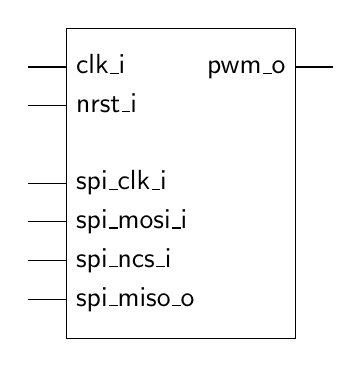
\begin{tikzpicture}
\draw  (2,0) rectangle (14,8);
\draw (0,7) -- (2,7) node [right] {\strut clk\_i};
\draw (0,6) -- (2,6) node [right] {\strut nrst\_i};
\draw (0,4) -- (2,4) node [right] {\strut spi\_clk\_i};
\draw (0,3) -- (2,3) node [right] {\strut spi\_mosi\_i};
\draw (0,2) -- (2,2) node [right] {\strut spi\_ncs\_i};
\draw (0,1) -- (2,1) node [right] {\strut spi\_miso\_o};
\draw (14,7) node [left] {\strut pwm\_o} -- (16,7);
\end{tikzpicture}
\caption{Top-level module symbol}
\end{figure}

\needspace{5\baselineskip}
\subsection{Ports description}

\begin{longtabu} to \textwidth {|X[1]|X[5]|}
\hline
\textbf{Port} & \textbf{Description} \\
\endfirsthead
\hline
\texttt{clk\_i} & Clock input \\
\hline
\texttt{nrst\_i} & Reset input (negative) \\
\hline
\texttt{spi\_clk\_i} & SPI clock \\
\hline
\texttt{spi\_mosi\_i} & SPI MOSI \\
\hline
\texttt{spi\_miso\_o} & SPI MISO \\
\hline
\texttt{spi\_ncs\_i} & SPI chip select \\
\hline
\caption{Module ports description}
\end{longtabu}

\section{Control interface}

The device is meant to be controller via SPI control interface. Each SPI transaction consists of two bytes: a command byte and a data byte.

\begin{figure}[h]
\centering
\begin{tikztimingtable}
MISO & 2{u}16{l}16{d}2{u} \\
MOSI & 2{u}16{d}{Command}16{d}2{u} \\
CLK  & 2{u}16{lh}2{u} \\
SS   & 2{h}32{l}2{h} \\
\end{tikztimingtable}
\caption{Generic SPI transaction}
\end{figure}

\begin{figure}[h]
\centering
\begin{tikztimingtable}
MISO & 2{u}16{l}16{d}{Readback}2{u} \\
MOSI & 2{u}2{h}14{d}{Read command}16{h}2{u} \\
CLK  & 2{u}16{lh}2{u} \\
SS   & 2{h}32{l}2{h} \\
\end{tikztimingtable}
\caption{SPI read diagram}
\end{figure}

\begin{figure}[h]
\centering
\begin{tikztimingtable}
MISO & 2{u}16{l}16{u}2{u} \\
MOSI & 2{u}2{l}14{d}{Write command}16{d}{Data}2{u} \\
CLK  & 2{u}16{lh}2{u} \\
SS   & 2{h}32{l}2{h} \\
\end{tikztimingtable}
\caption{SPI write diagram}
\end{figure}

\begin{figure}[h]
\centering
\begin{tikztimingtable}[timing/wscale=4]
MOSI & 2{u}2{d}{R/W}10{d}{Channel}4{d}{Reg}d \\
CLK  & 2{u}8{lh}l \\
SS   & 2{h}16{l}l \\
\end{tikztimingtable}
\caption{Command structure}
\end{figure}

\begin{longtabu} to \textwidth {|X[1]|X[5]|}
\hline
\textbf{Field} & \textbf{Description} \\
\endfirsthead
\hline
\texttt{RW[7]} & Read/write. Set to 1 when performing a read transaction. \\
\hline
\texttt{CH[6:2]} & Channel. Refers to instance of \texttt{pwm} module within the top-level architecture. \\
\hline
\texttt{ADDR[1:0]} & Target register address. \\
\hline
\caption{Command structure}
\end{longtabu}

\section{Register map}

\begin{longtabu} to \textwidth{|X[1]|X[5]|}
\hline
\textbf{Address} & \textbf{Description} \\
\endfirsthead
\hline
\texttt{0x00} & Control register \\
\hline
\texttt{0x01} & Duty cycle upper byte \\
\hline
\texttt{0x02} & Duty cycle lower byte \\
\hline
\caption{Register address mapping}
\end{longtabu}

\needspace{20\baselineskip}
\begin{regtable}{Control register}
Field & EN & \multicolumn{5}{c|}{---} & \multicolumn{2}{c|}{DEV}\\
\hline
Default & 0 & \multicolumn{5}{c|}{---} & \multicolumn{2}{c|}{00}\\
\hline
R/W & RW & \multicolumn{5}{c|}{---} & \multicolumn{2}{c|}{RW}\\
\hline
~ & 7 & 6 & 5 & 4 & 3 & 2 & 1 & 0 \\
\end{regtable}

\begin{longtabu} to \textwidth {|X[1]|X[5]|}
\hline
\textbf{Field} & \textbf{Description} \\
\endfirsthead
\hline
EN & Enable \texttt{pwm} instance \\
\hline
DEV & Set duty cycle deviation \\
\hline
\caption{Control register fields}
\end{longtabu}

\begin{regtable}{Duty cycle upper byte}
Field & \multicolumn{6}{c|}{---} & \multicolumn{2}{c|}{DC[9:8]}\\
\hline
Default & \multicolumn{6}{c|}{---} & \multicolumn{2}{c|}{00}\\
\hline
R/W & \multicolumn{6}{c|}{---} & \multicolumn{2}{c|}{RW}\\
\hline
~ & 7 & 6 & 5 & 4 & 3 & 2 & 1 & 0 \\
\end{regtable}

\begin{regtable}{Duty cycle lower byte}
Field & \multicolumn{8}{c|}{DC[7:0]} \\
\hline
Default & \multicolumn{8}{c|}{00000000} \\
\hline
R/W & \multicolumn{8}{c|}{RW} \\
\hline
~ & 7 & 6 & 5 & 4 & 3 & 2 & 1 & 0 \\
\end{regtable}

\end{document}
